%%% Содержимое слайдов

% 1. Название, автор, руководитель.
% 2. Постановка задачи (актуальность)
% 3. способ (инструменты для) решения
% 4. результаты
% 5. анализ результатов
% 6. Заключение 

\frame[plain]{\titlepage} % Титульный слайд

%-------------------------------------------------------------------------------

\section{Постановка задачи}

\begin{frame}
\frametitle{\insertsection}

\begin{itemize}    
    \item Решение полных постановок задач весьма ресурсоемко
    \item Задача разработки метода решения прямой задачи БКЗ
    \item Решение математической постановки прямой задачи БКЗ неэффективно уже имеющимися средствами
\end{itemize}
\end{frame}

%-------------------------------------------------------------------------------

\section{Способ решения}

\begin{frame}
\frametitle{\insertsection}

\textbf{Инструменты:}
\begin{itemize}
    \item Язык программирования Python
    \item Вычислительная платформа FEniCS
    \item Модуль triangle для триангуляции Делоне
    \item Компьютер: ОС Ubuntu 18.04 LTS, процессор Intel Pentium 4415U 2.30 ГГц
\end{itemize}
\end{frame}

%-------------------------------------------------------------------------------

\section{Результаты}

\begin{frame}
\frametitle{\insertsection}

\vspace{-0.5cm}
\begin{minipage}[t]{0.47\linewidth}
    \textbf{Модель 1}
    \center{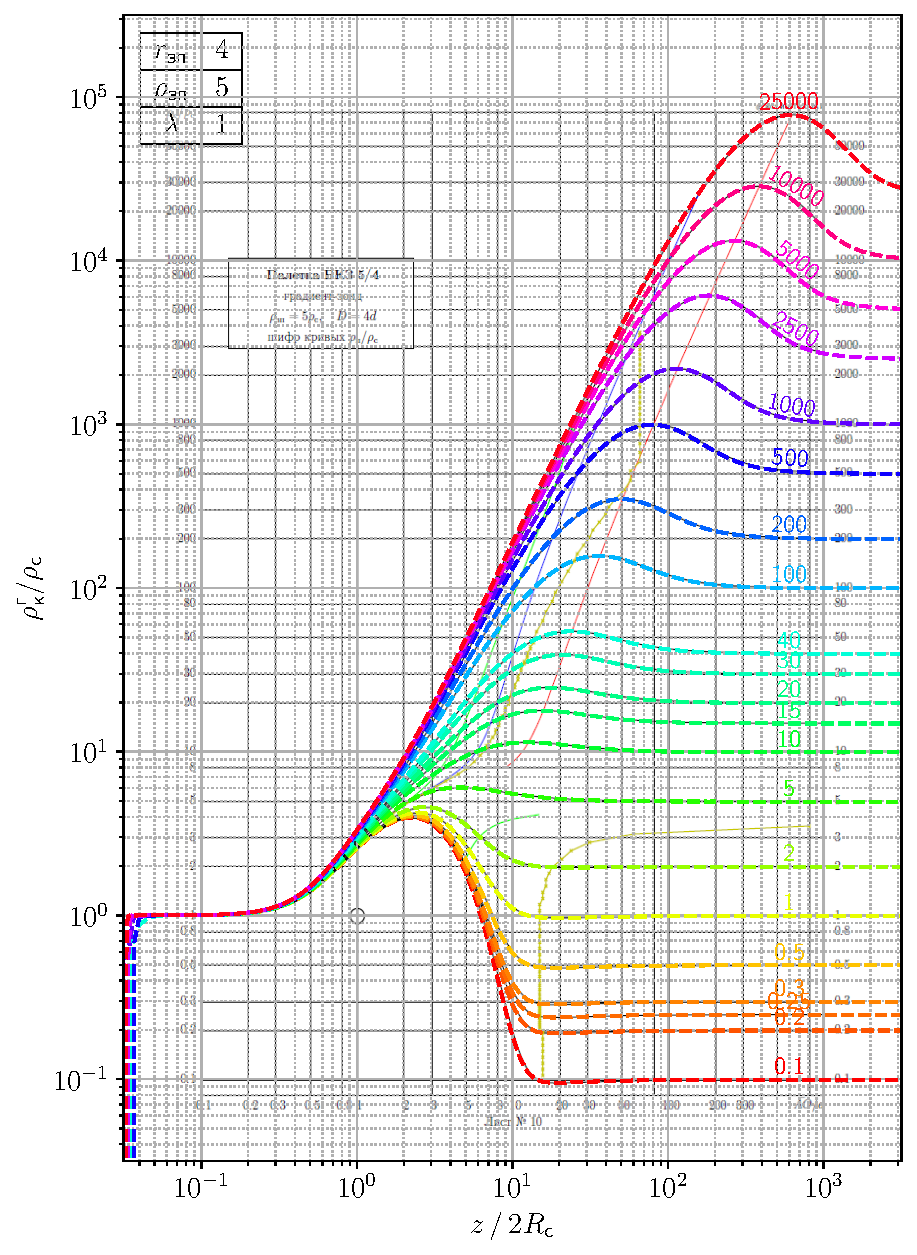
\includegraphics[width=1\linewidth]{plot_1_compare}}
\end{minipage}
\hfill
\begin{minipage}[t]{0.47\linewidth}
    \textbf{Модель 2}
    \center{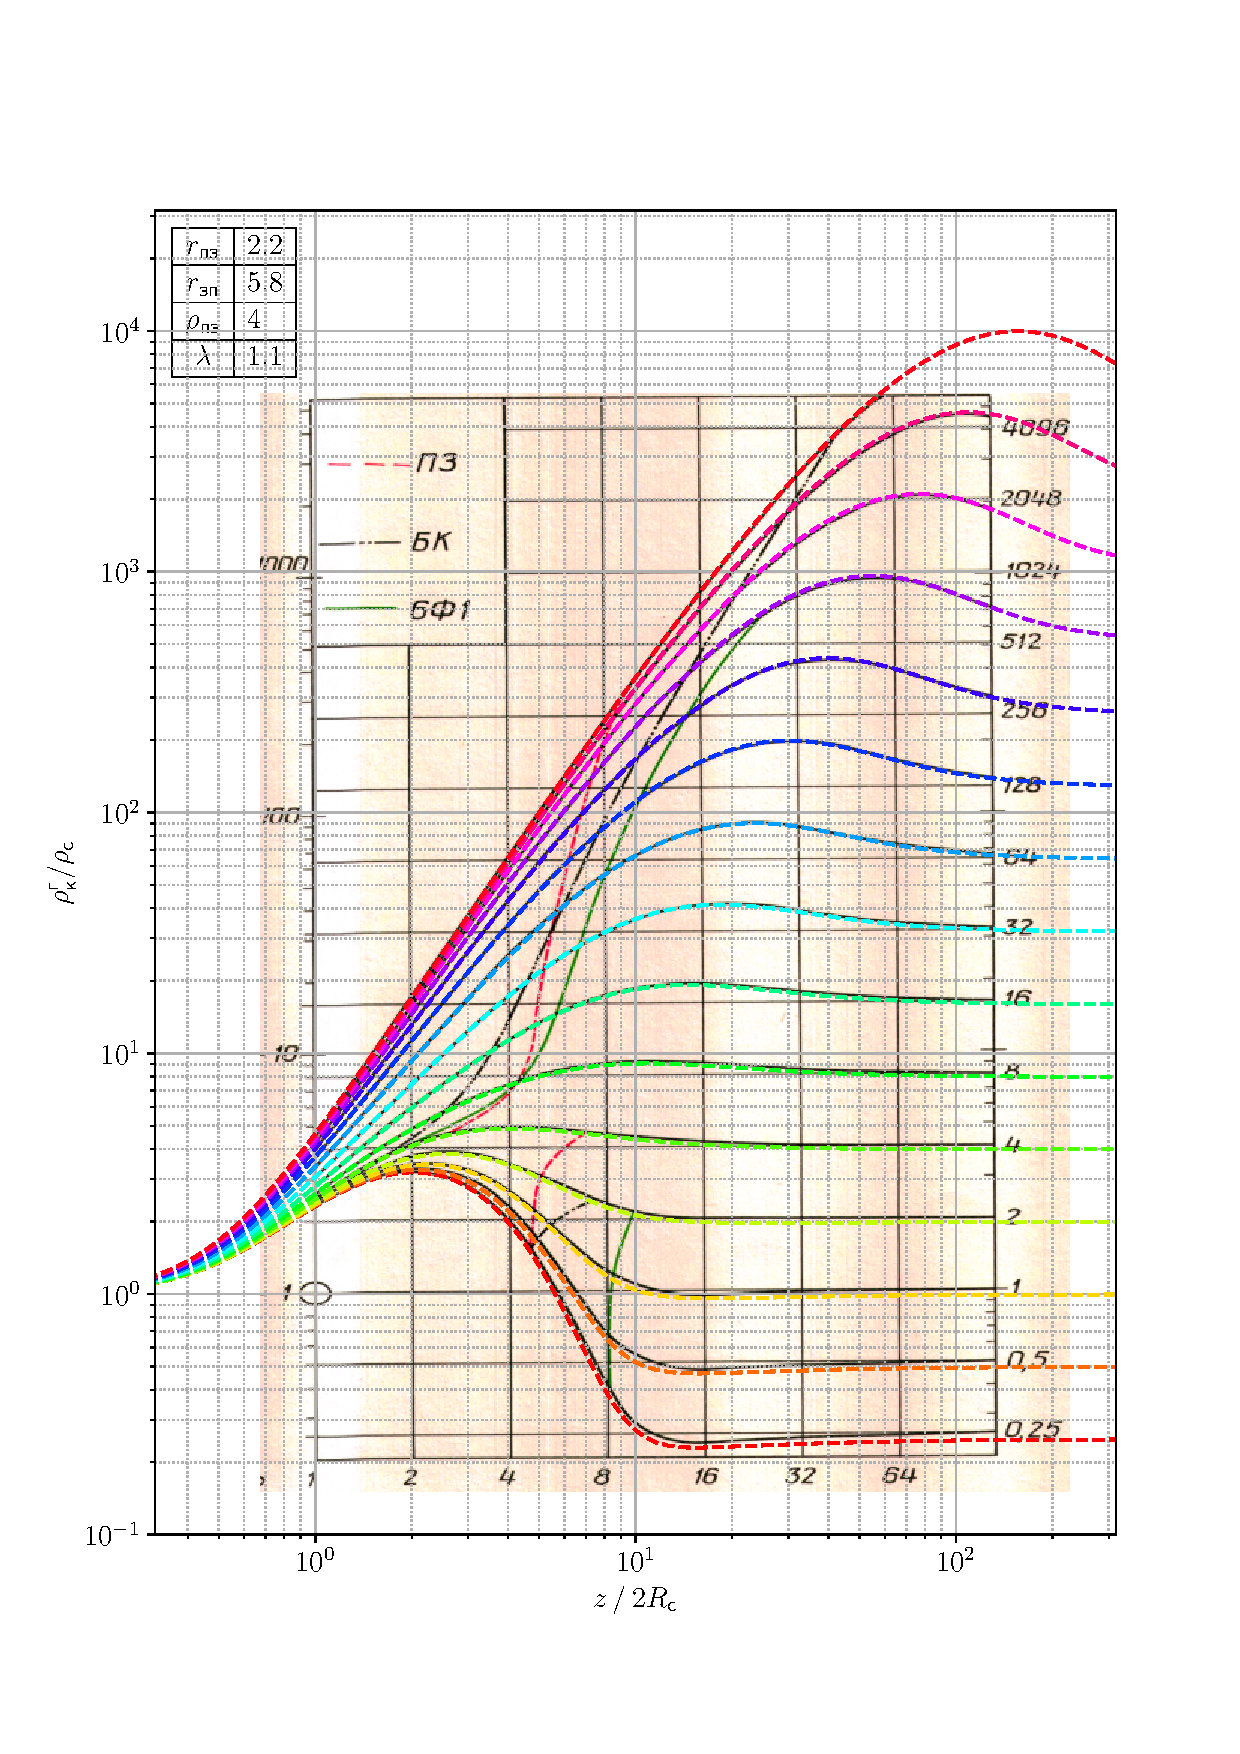
\includegraphics[width=1\linewidth]{plot_2_compare}}
\end{minipage}

\end{frame}

%-------------------------------------------------------------------------------

\section{Анализ результатов}

\begin{frame}
\frametitle{\insertsection}

\textbf{Модель 1:}
\begin{itemize}
    \item Время вычисления расчетной палетки ${18 \text{ c } \pm 159 \text{ мс }}$, 7 проходов
\end{itemize}

\textbf{Модель 2:}
\begin{itemize}
    \item Время вычисления расчетной палетки ${16.5 \text{ c } \pm 176 \text{ мс}}$, 7 проходов
\end{itemize}

\textbf{Критерии точности решения}:
\begin{itemize}
    \item гладкость решения
    \item сравнение "на глаз" решения с известным
\end{itemize}
\end{frame}

%-------------------------------------------------------------------------------

\section{Заключение}

\begin{frame}
\frametitle{\insertsection}

\begin{itemize}
    \item Освоены пакеты программ для параллельных вычислений
    \item Проведены расчеты и сопоставление с известными результатами в литературе
    \item Показана применимость метода решения прямой задачи БКЗ
\end{itemize}
\end{frame}

%-------------------------------------------------------------------------------

\section{Конец}

\begin{frame}
\centering
\vfill
\textcolor{Blue}{\Large Спасибо за внимание!}
\vfill
\end{frame}